\section{Finding An Optimal Solution}

Now that I have derived the general formula for the length of the garland and convinced myself that it is correct, I can now devise a way to meet my objective of meeting personal aesthetic preferences while minimizing waste. This is because the height $H$ and radius $R$ of the tree is fixed, and as such the spacing between successive rotations of the garland $\lambda$ is the only parameter which could theoretically be optimized.

The first thing I did was to check whether $L(\lambda, R, H)$ had any minima. This is because if there were minima for the multivariate equation, whether global or local, this would mean that for certain values of $R$ and $H$, there would exist optimal solution(s) for $\lambda$ which result in shorter lengths of garland than other values of $\lambda$ in their neighborhood, which would mean less garland used and thus less waste. One way that I could check for minima is to evaluate the partial derivatives of $L(\lambda, R, H)$ with respect to each of the 3 parameters $\lambda$, $R$, and $H$, and set them equal to zero. i.e. $\pdv{L}{\lambda} = 0$, $\pdv{L}{R} = 0$, and $\pdv{L}{H} = 0$. This would give me 3 equations, and I could solve the system of equations to obtain values of $\lambda$, $R$, and $H$ which would correspond to the critical points that could potentially be minima. However, given the complexity of the partial derivatives, it is probably very difficult or outright impossible to obtain a solution analytically. I would instead need to find a way to evaluate this numerically, and so I turned to \emph{Wolfram Alpha}, which promptly told me that the equation in fact had no global or local minima at all.  Thus, there are never any situations where certain values of $\lambda$ are objectively more optimal in that it uses less garland than other $\lambda$ values in its neighborhood, and as such I will have turn to more subjective means to define what I mean by ``optimal'' solutions.
\begin{figure}[H]
    \centering
    \begin{subfigure}[t]{0.7\textwidth}
        \centering
        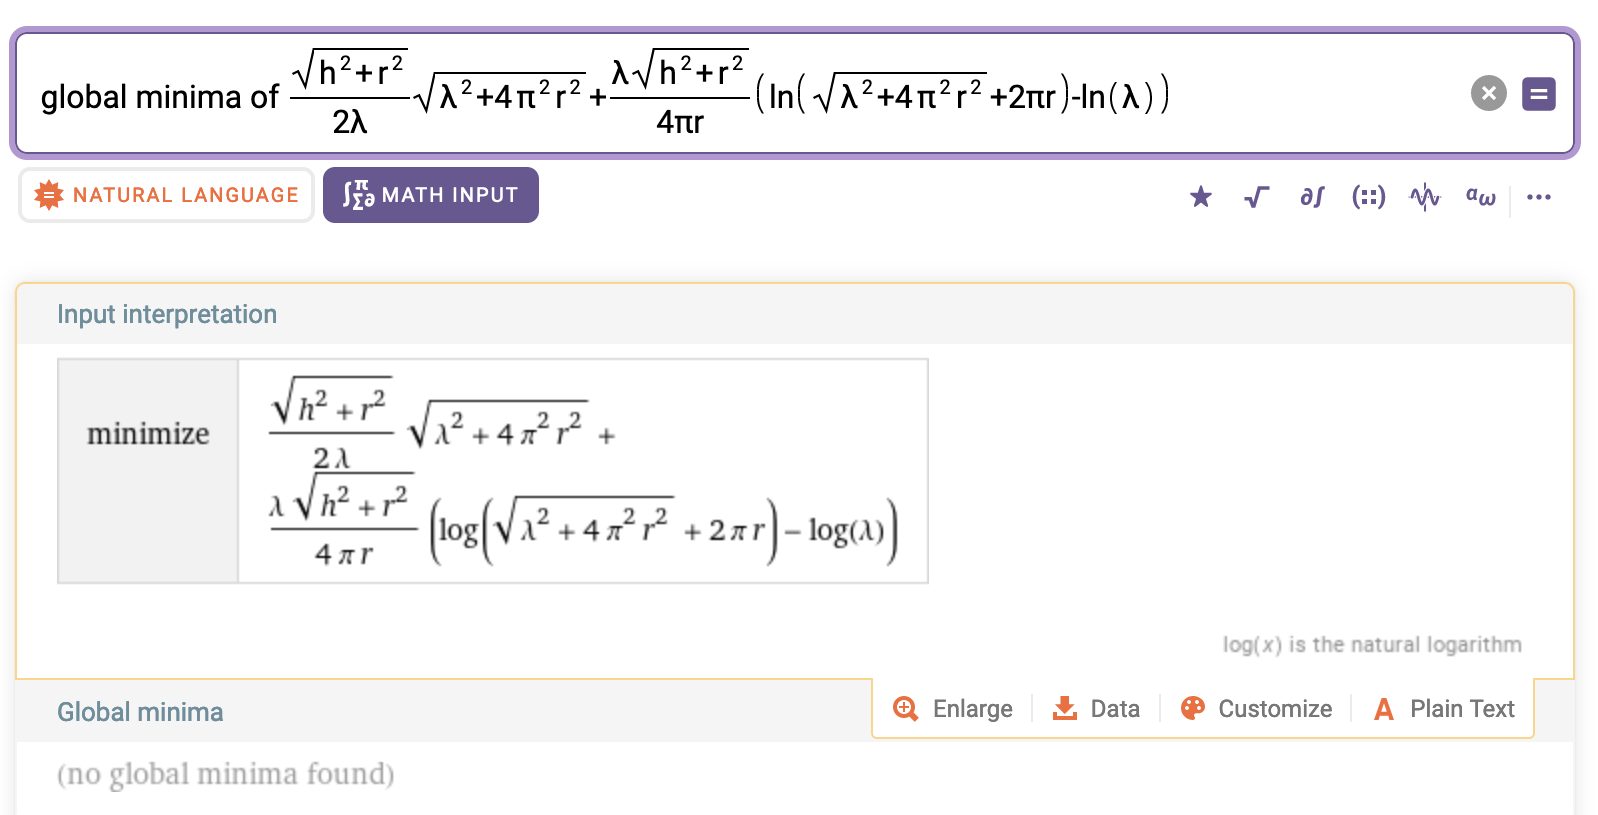
\includegraphics[width=\textwidth]{images/wolfram_global_minima.png}
    \end{subfigure}
\end{figure}
\begin{figure}[H]\ContinuedFloat
    \centering
    \begin{subfigure}[t]{0.7\textwidth}
        \centering
        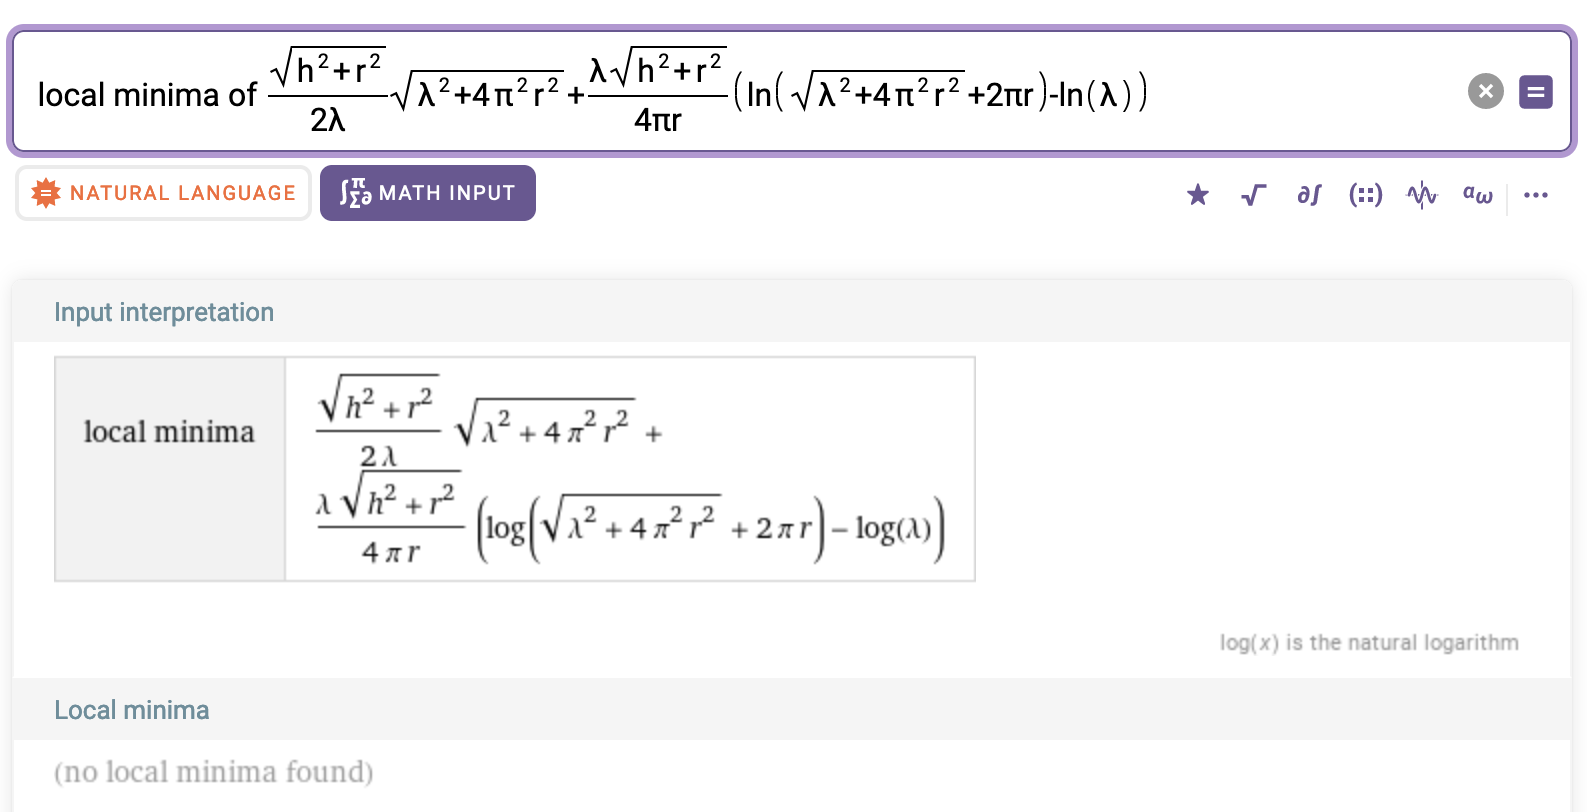
\includegraphics[width=\textwidth]{images/wolfram_local_minima.png}
    \end{subfigure}
    \caption{The equation has no global or local minima, according to \emph{Wolfram Alpha}.}
    \vspace*{-10pt}
\end{figure}

Given that there are no globally optimal solutions, I decided that I should instead focus on my particular Christmas tree, which has the dimensions $R=\US{15}{\inch}$ and $H=\US{72}{\inch}$. I realized it was important to first understand the dynamics of the function, and so I graphed the function in \emph{Desmos}, with $\lambda$ as the independent variable and $L$ as the dependent variable, as visualized in Figure \ref{fig:graph}. Firstly, I noted that the function was decreasing over the entire domain, meaning that as $\lambda$ increases, the length of garland required $L$ decreases. This is reasonable, given that larger spacing between successive rotations of the garland would mean that garland would have to go around the tree a lesser amount of times before it reaches to the tip of the tree, and thus mean that a shorter length of garland is necessary.
\begin{figure}[H]
    \vspace*{5pt}
    \centering
    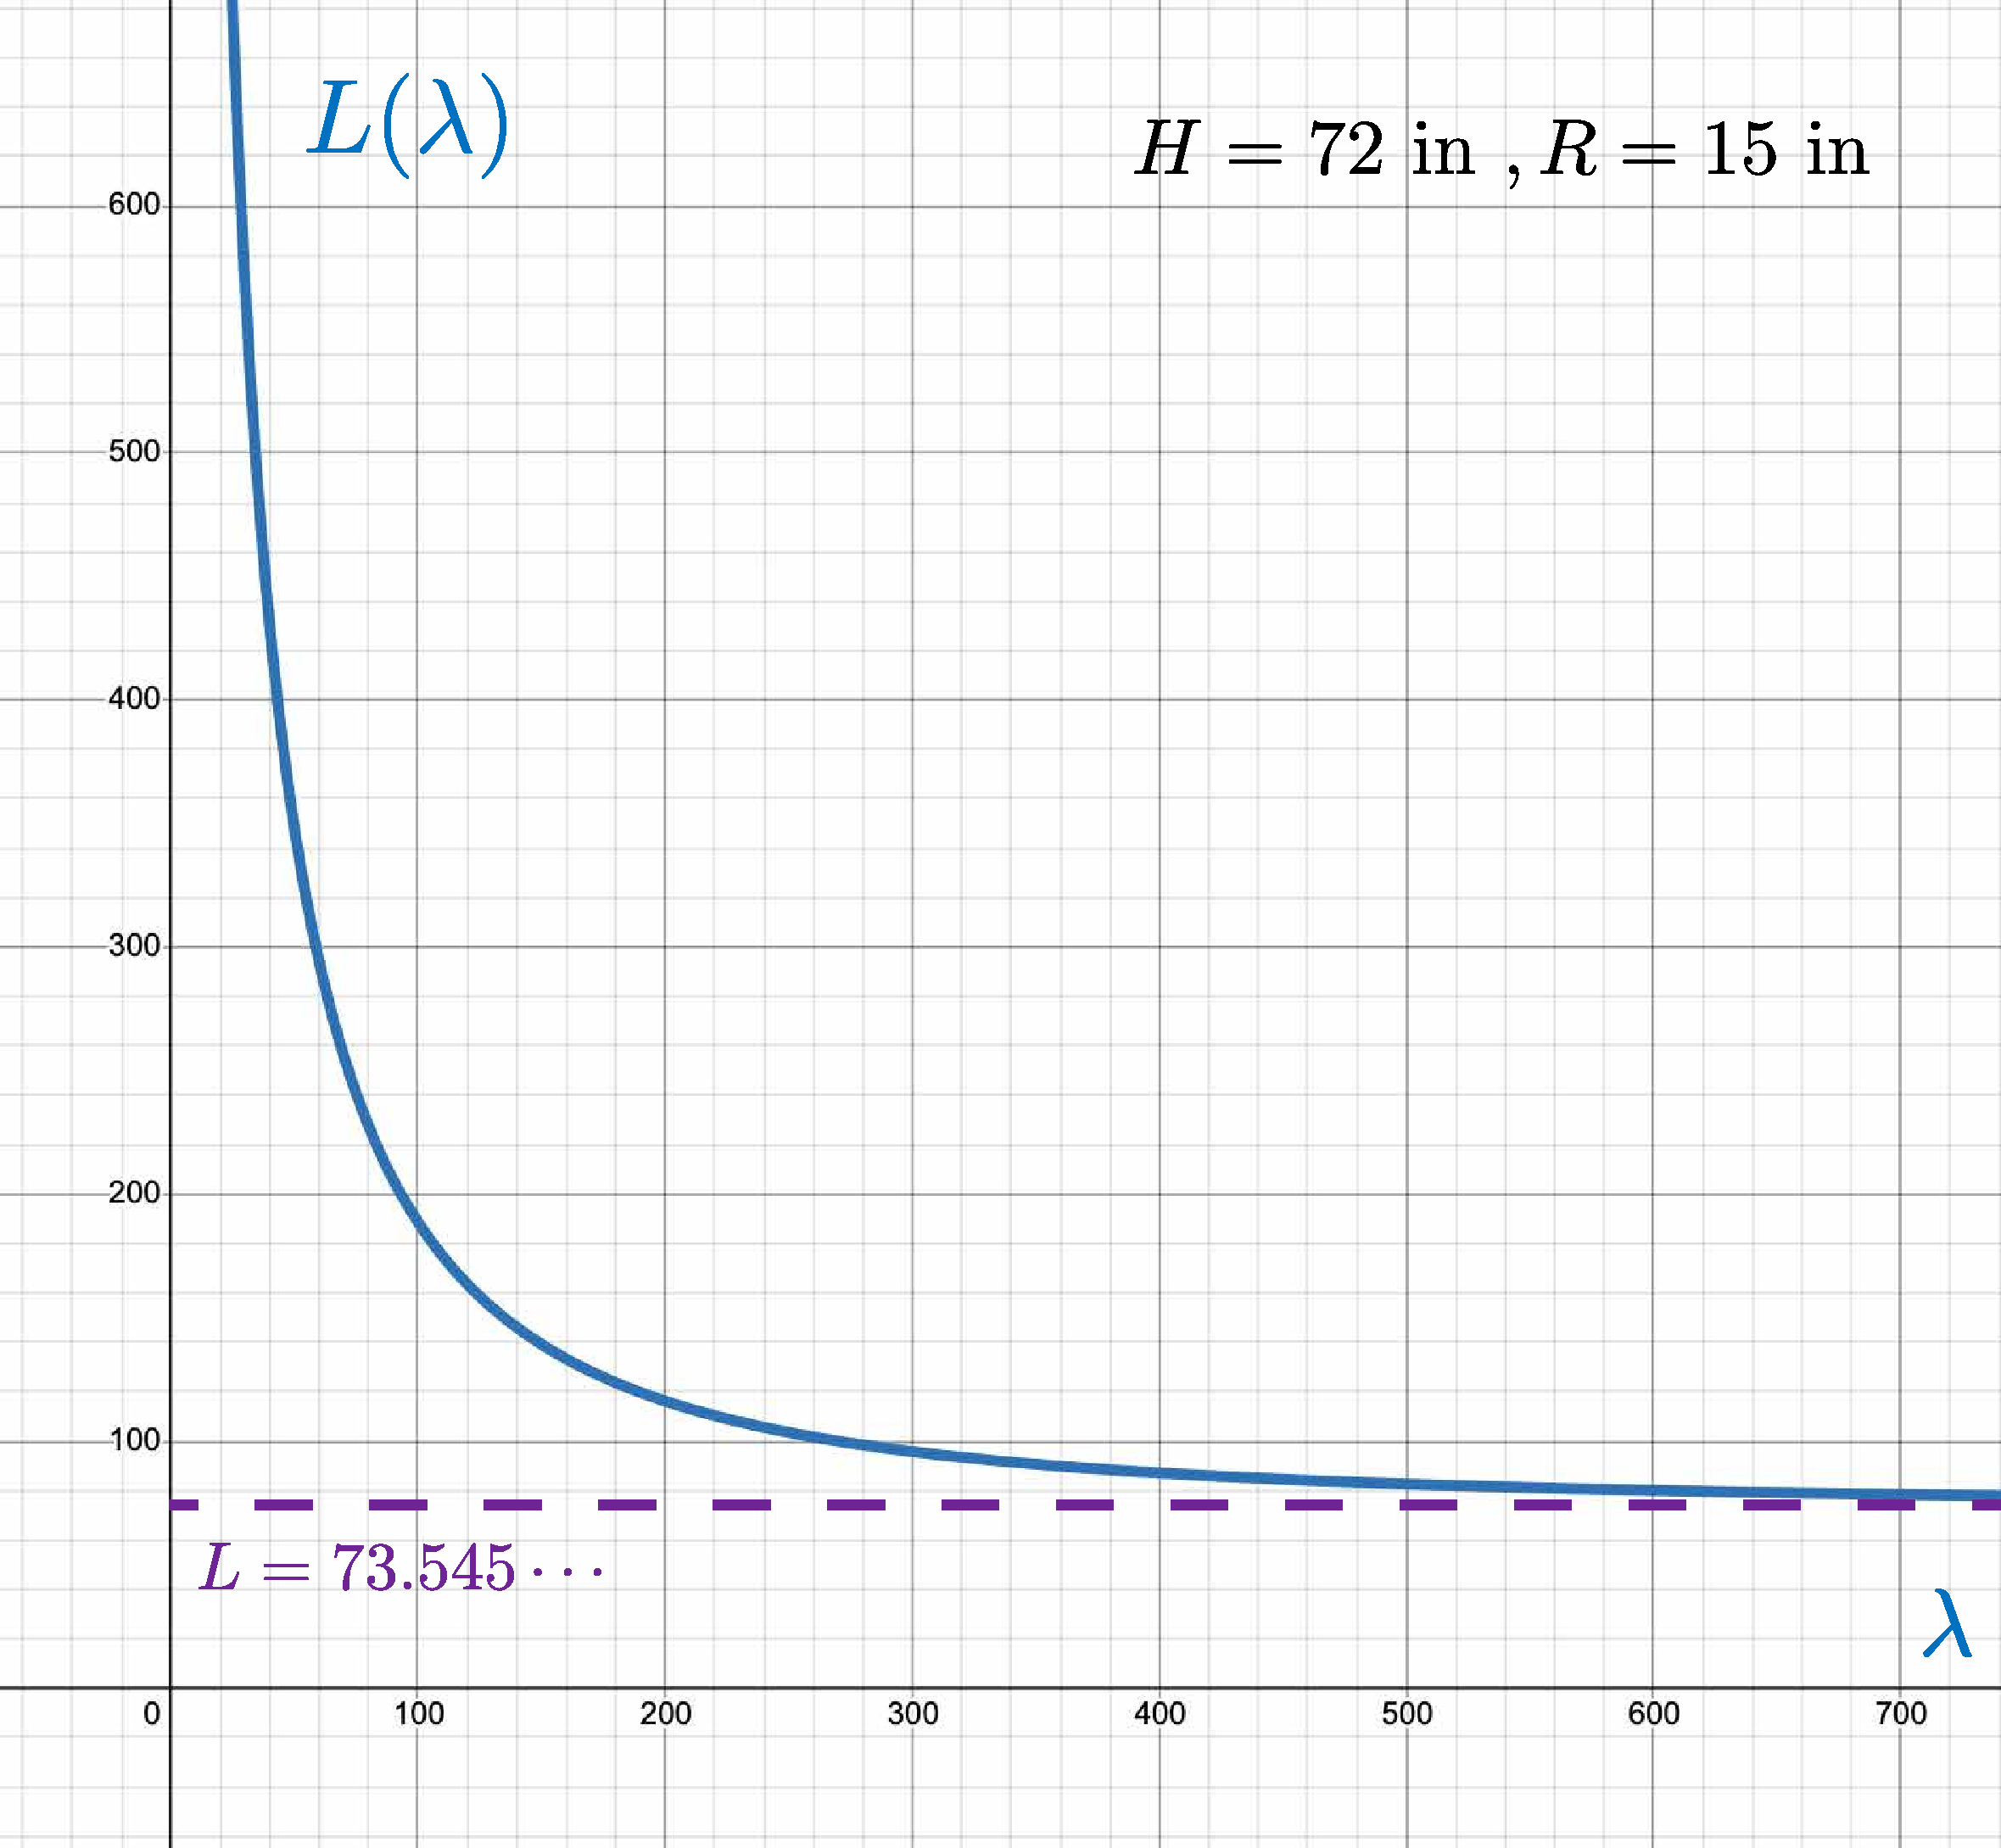
\includegraphics[width=0.5\textwidth]{diagrams/graph.pdf}
    \caption{Graph of $L$ vs. $\lambda$ with $H=\US{72}{\inch}$ and $R=\US{15}{\inch}$} \label{fig:graph}
    \vspace*{-15pt}
\end{figure}
\noindent Another interesting thing to note is that the function is asymptotic, because from the graph we can see that as $\lambda \rightarrow +\infty$, $L$ converges towards $L = \US{73.5459}{\inch}$, which is the slant height of the cone ($\sqrt{15^2+72^2} = 73.5459\cdots$). In fact, I prove in Appendix \ref{sec:qzhsb} that:
\begin{equation}
    \lim_{\lambda \to +\infty} L(\lambda, R, H) = \sqrt{R^2+H^2} \qquad \forall R, H \in \Real^+
\end{equation}
which is the slant height of the tree. This makes sense, given that the shortest length possible for the garland would be a straight line from the tip of the tree to the bottom of the tree, which would be equal to the slant height. Finally, we see that as $\lambda$ decreases, the amount garland needed exponentially increases. Thus, while I want to space the garland such that the tree look nice according to my personal preferences, it is also important not to choose a spacing too small, as it would require a lot more garland, and not only is that wasteful and unnecessary spending, it is harmful to the environment as I will be using plastic tinsel garland.

Since the function does not have minima, I will have to subject to additional requirements in order to arrive at ``optimal'' solution(s). One thing I quickly realized was that the function was continuous, but in reality garland is typically sold in standard unit lengths; for example, the garland which my family bought is sold in $\US{6}{\feet}$ lengths (or $\US{72}{\inch}$). This means that the amount of garland that I buy can only be a positive multiple of unit lengths of garland, which can mathematically represented thus:
\begin{equation}
    L_G = nG,\quad n \in \Integer^+ \label{eq:nG}
\end{equation}
where $L_G$ denotes the total length of garland required, $G$ represents the individual unit lengths of the garland, and $n\in \Integer^+$ is the number of lengths of garland that I need to buy. As such, if I wanted to minimize wasted and have as little excess garland as possible, I would want the theoretical minimum amount of garland, $L$, to be roughly equal to some multiple of $G$, i.e. $L(\lambda, R, H) = nG$.
and find solutions for $\lambda$
My initial approach was to equate $L(\lambda, R, H)$ to $nG$ and isolate for $\lambda$. I could then input positive integers into $n$ to get all possible values for $\lambda$ which result in lengths of the garland that are multiples of $G$. However, I quickly realized that this was not viable, as the complexity of the equation from the square roots and the logarithms means that it is very difficult or most likely impossible to isolate for $\lambda$. As such, this problem will have to be solved numerically.




Given that we know the value of $G=\US{72}{\inch}$, we can calculate the amount of garland necessary, $n$, by dividing $L$ by $G$, and rounding up the result to a whole number. This can be mathematically represented using the ceiling function:
\begin{equation}
    n = \left\lceil \frac{L(\lambda, R, H)}{G} \right\rceil
\end{equation}
Plugging this for $n$ in equation \ref{eq:nG}, we get that:
\begin{equation}
    L_G(\lambda, R, H) = G\left\lceil \frac{L(\lambda, R, H)}{G} \right\rceil
\end{equation}

Using this, I can graph $L_G$ and compare it to $L$.
\begin{figure}[H]
    \centering
    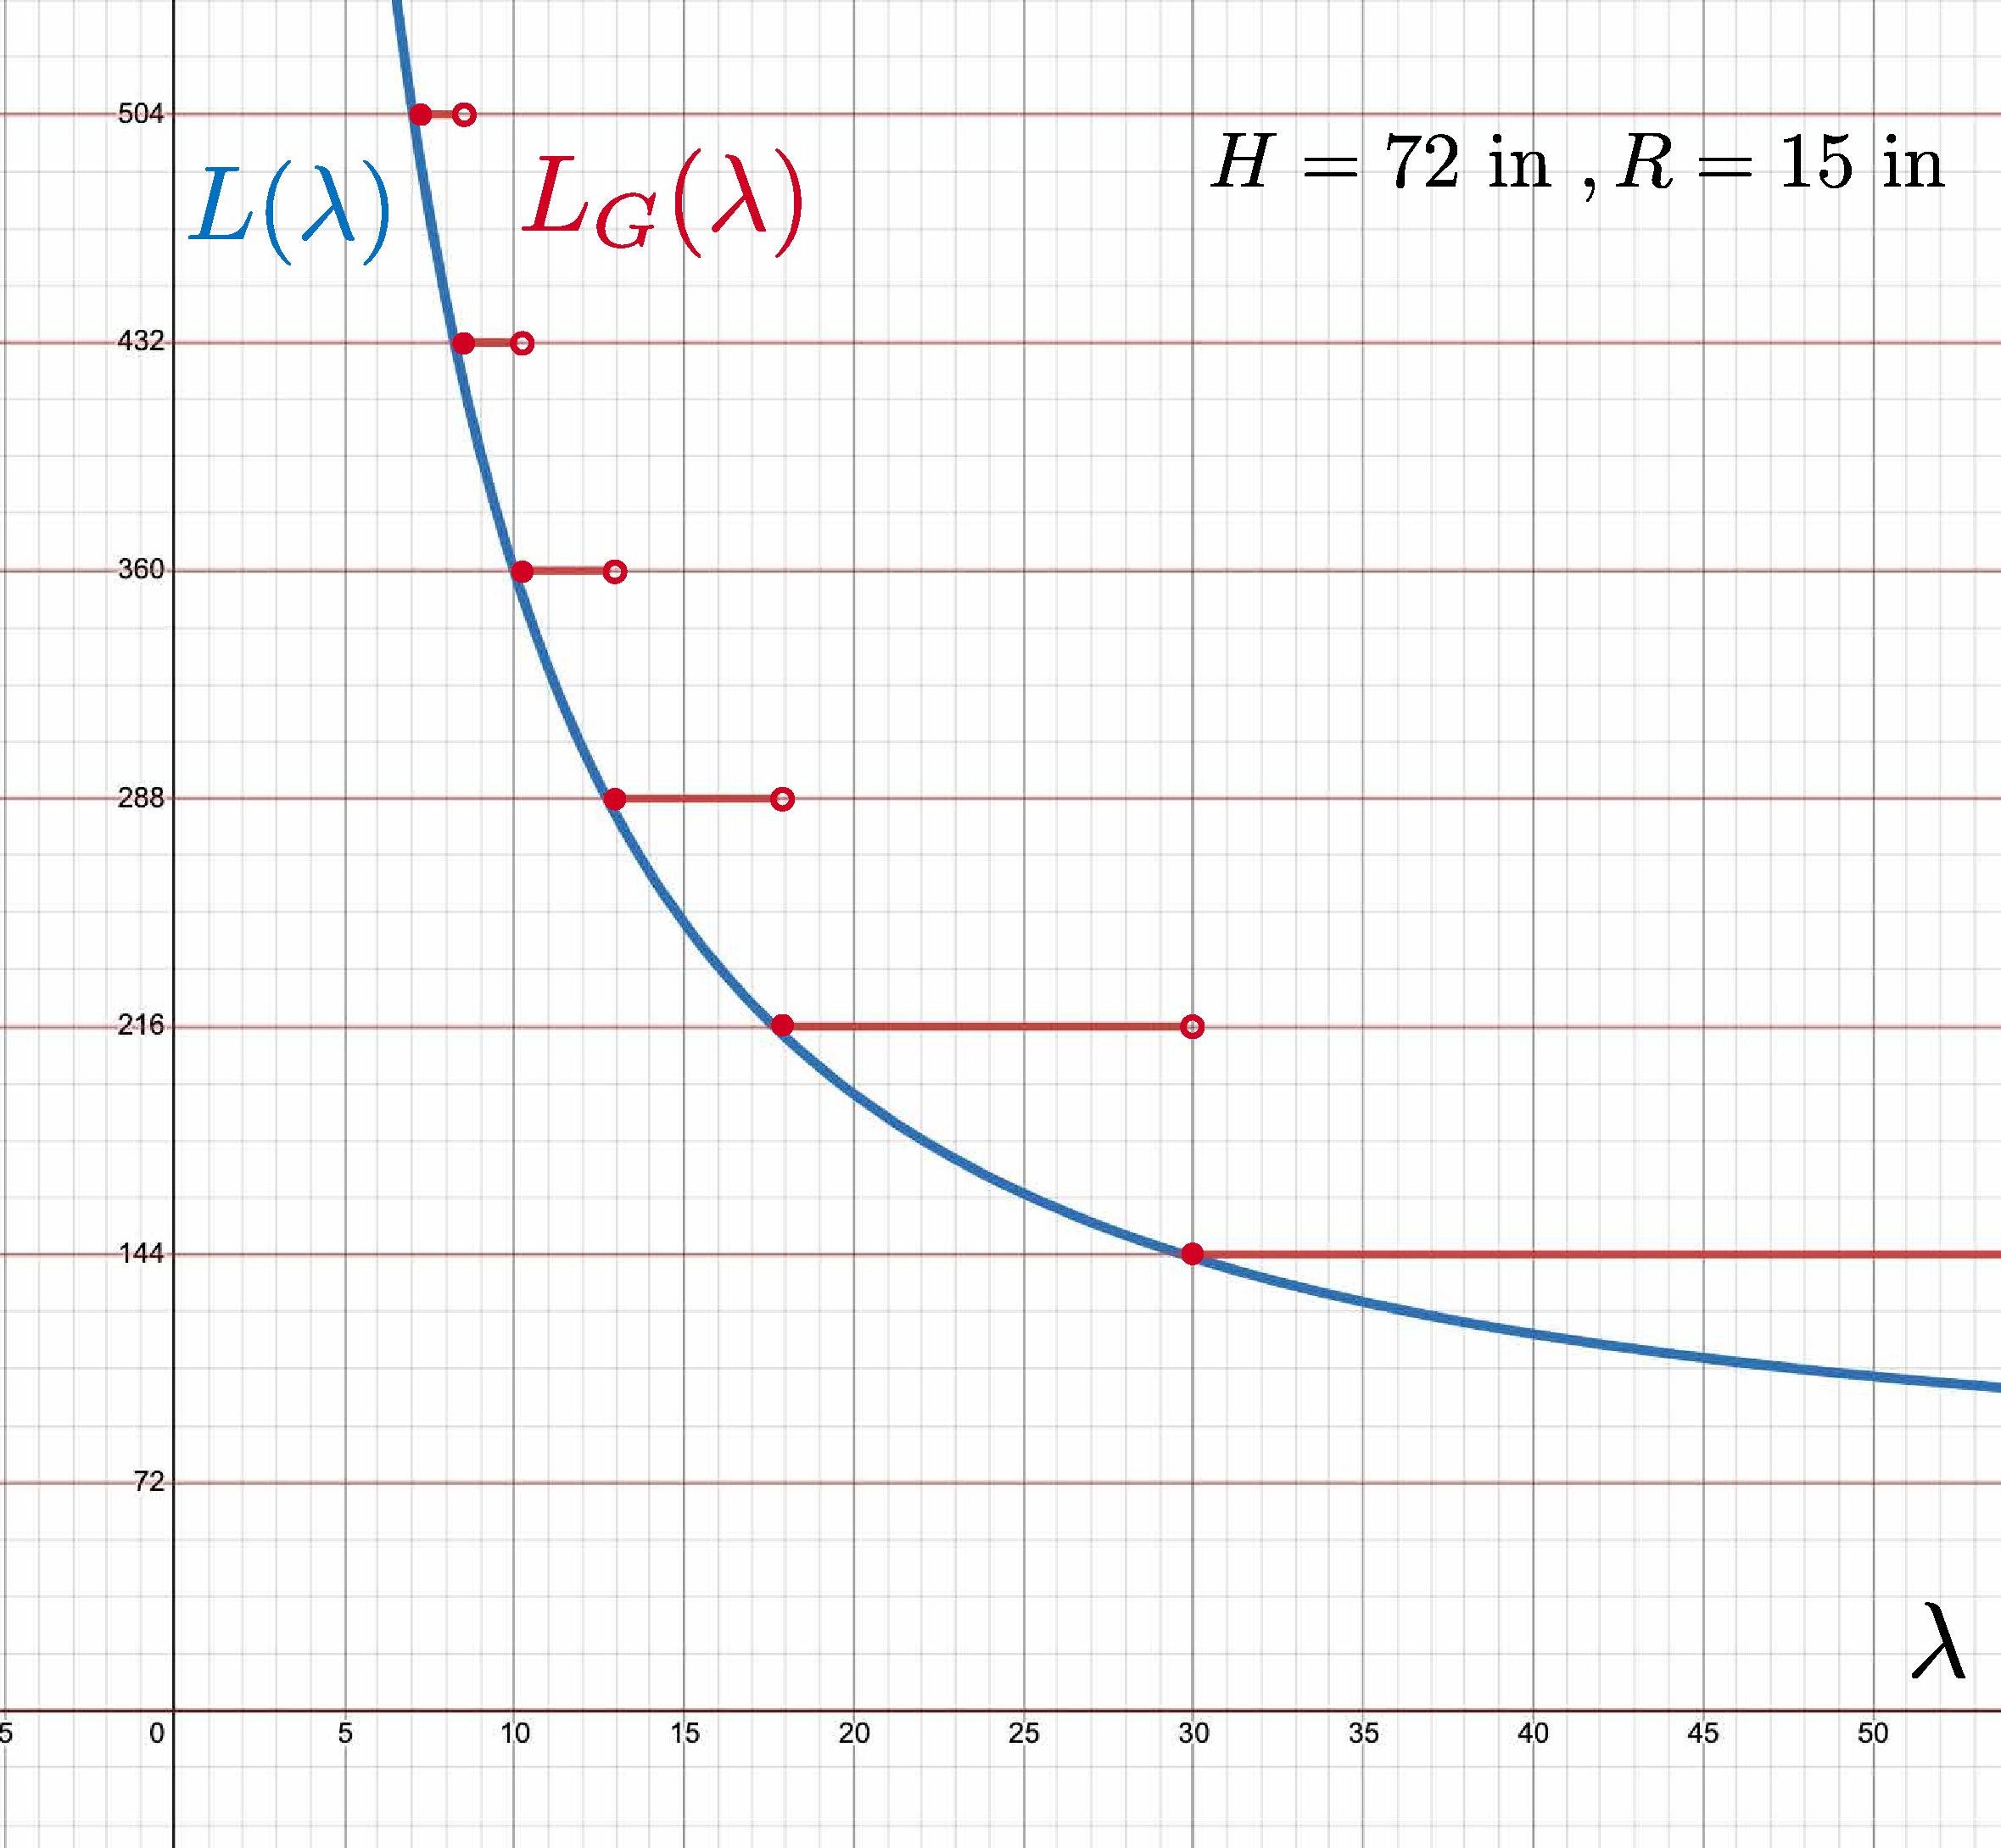
\includegraphics[width=0.6\textwidth]{diagrams/step_comparison.pdf}
    \caption{A comparison between $L$ and $L_G$.}
\end{figure}



\begin{figure}[H]
    \centering
    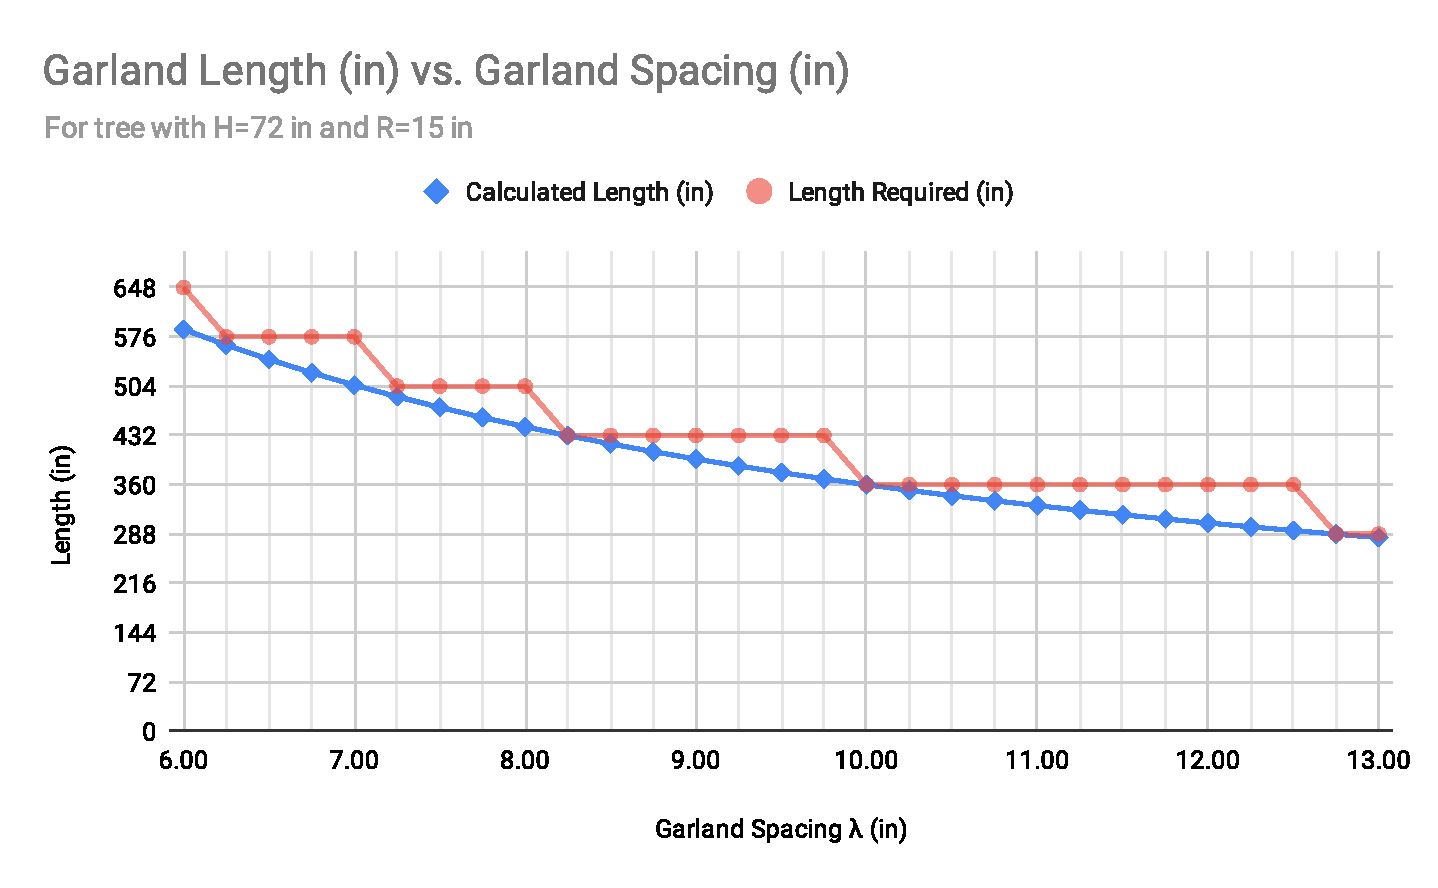
\includegraphics[width=0.8\textwidth]{diagrams/detailed_graph.pdf}
    \caption{Graph showing the length of garland $L$ vs. the garland spacing $\lambda$.  (Generated using \emph{Google Sheets})}
\end{figure}

The fact that garland is sold in unit lengths means that there will almost always be some lengths of garland which will be excess unless the theoretical garland length $L$ calculated by my general formula is exactly equal to $L_G$.

\begin{figure}[H]
    \centering
    \begin{subfigure}[t]{0.15\textwidth}
        \centering
        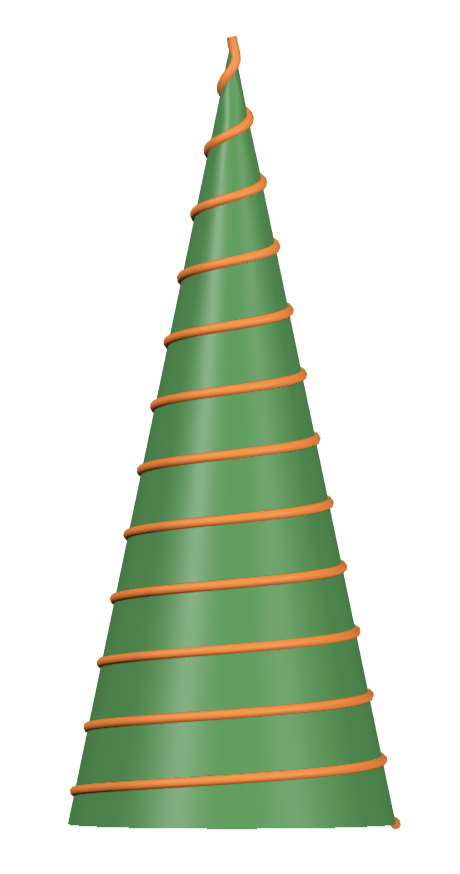
\includegraphics[width=\textwidth]{images/garland_spacings/6in.png}
        \caption{$\US{6}{\inch}$ Spacing.}
    \end{subfigure}
    \hspace*{0.05\textwidth}
    \begin{subfigure}[t]{0.15\textwidth}
        \centering
        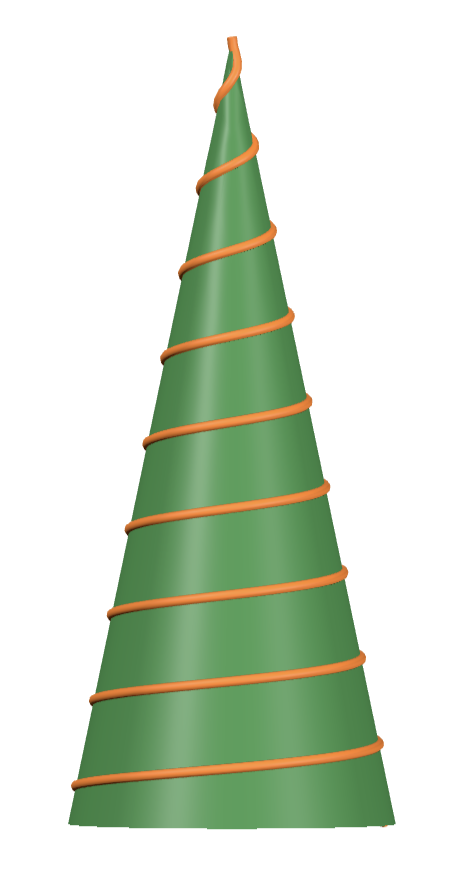
\includegraphics[width=\textwidth]{images/garland_spacings/8in.png}
        \caption{$\US{8}{\inch}$ Spacing.}
    \end{subfigure}
    \hspace*{0.05\textwidth}
    \begin{subfigure}[t]{0.15\textwidth}
        \centering
        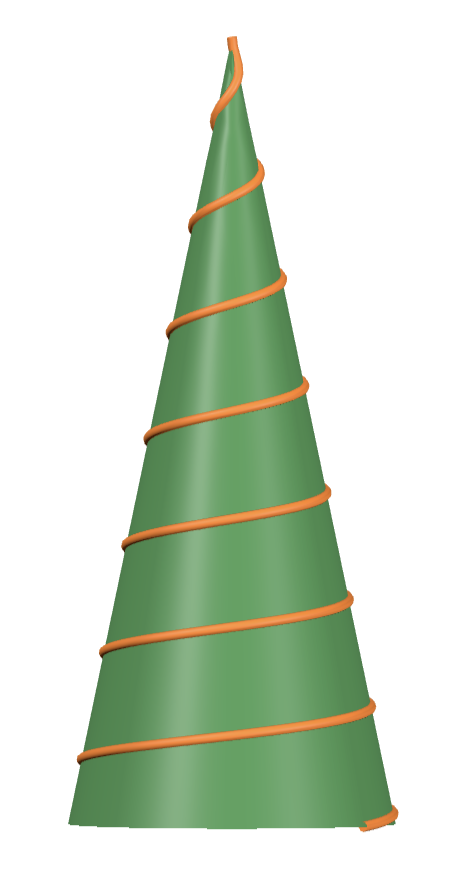
\includegraphics[width=\textwidth]{images/garland_spacings/10in.png}
        \caption{$\US{10}{\inch}$ Spacing.}
    \end{subfigure}
    \hspace*{0.05\textwidth}
    \begin{subfigure}[t]{0.15\textwidth}
        \centering
        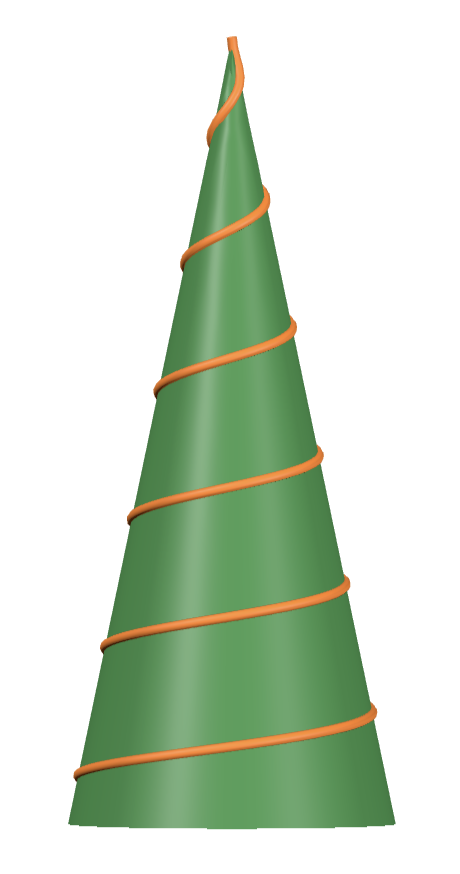
\includegraphics[width=\textwidth]{images/garland_spacings/12in.png}
        \caption{$\US{12}{\inch}$ Spacing.}
    \end{subfigure}
    \caption{Comparison between different spacing for the garland. }
\end{figure}
